\documentclass[a4paper,french,towsides,10pt]{book}
\usepackage[utf8]{inputenc}
\usepackage[french]{babel}
\usepackage{fancyhdr}
\usepackage{enumerate}
\usepackage{graphicx}
\usepackage{glossary}
\usepackage[french]{minitoc}
\usepackage{multirow}
\usepackage{placeins}
\usepackage{listings}
\usepackage{color}
\usepackage{float}
\usepackage{tabularx}
\usepackage[english,ruled,vlined,linesnumbered]{algorithm2e}
\usepackage{amsmath}
\usepackage{amssymb}
\usepackage[french]{varioref}
\usepackage[bookmarks=true]{hyperref}

\hypersetup{pdfborder={0 0 0}}
\pagestyle{fancy}
\setlength{\parskip}{1.5ex plus .4ex minus .4ex}
\renewcommand{\labelitemi}{\textbullet}
\renewcommand{\chaptermark}[1]{\markboth{#1}{}}


\def\doctitle{Intelligence artificielle : une approche cognitive}

\def\cogito{\emph{\mbox{COGITO}}}

\newcommand{\method}[1]{\texttt{{#1}}}
\newcommand{\class}[1]{\texttt{{#1}}}
\newcommand{\package}[1]{\textbf{{#1}}}
\newcommand{\gls}[1]{\newgls{#1}}


\pagestyle{fancy}

\renewcommand{\chaptermark}[1]{\markboth{#1}{}}
\renewcommand{\sectionmark}[1]{\markright{\thesection\ #1}}

\fancyhf{}

\fancyhead[RO,LE]{\thepage}
\fancyhead[LO]{\leftmark}
\fancyhead[RE]{\doctitle}

\fancypagestyle{corps}{ 
\fancyhead[RO,LE]{\thepage}
\fancyhead[LO]{\rightmark}
\fancyhead[RE]{\leftmark}
}

\renewcommand{\footrulewidth}{0pt} % pas de filet en bas
\fancypagestyle{plain}{ % pages de tetes de chapitre
\fancyhead{}
% supprime l’entete
\renewcommand{\headrulewidth}{0pt} % et le filet
}
\newcommand{\clearemptydoublepage}{%
	\newpage{\pagestyle{empty}\cleardoublepage}}


%Modification des marges
%\\oddsidemargin}{-2,5cm}
%\addtolength{\textwidth}{5cm}
%\addtolength{\topmargin}{-2,5cm}
%\addtolength{\textheight}{4cm}

%definition des fonctions de la page de garde
\def\blurb{%
  \begin{tabular}{l p{0.6cm} c p{0.8cm} r}
   \multirow{3}{*}{\vspace{-1.5cm}\hspace{-1cm}
\includegraphics[width=3cm]{./files/um2}} & & & &  \multirow{3}{*}{\vspace{-1.5cm}
\includegraphics[width=2cm]{./files/ufr}} \\
    & & Ministère de l'Éducation Nationale & & \\
    & & Université de Montpellier II & & \\ 
    & & Place Eugène Bataillon & & \\ 
    & & 34095 Montpellier Cedex 5 & & \\
    & & & & \\
    & & Rapport final du TER GMIN20B & & \\
    & & du Master Informatique 1\iere année, & & \\
    & & effectué de Janvier à Mai 2012 & & \\
    & & et encadré par Violaine \textsc{Prince} & & \\
    \vspace{0.5cm}
   \end{tabular}
  }
\def\clap#1{\hbox to 0pt{\hss #1\hss}}%
\def\ligne#1{%
  \hbox to \hsize{%
    \vbox{\centering #1}}}%
\def\haut#1#2#3{%
  \hbox to \hsize{%
    \rlap{\vtop{\raggedright #1}}%
    \hss
    \clap{\vtop{\centering #2}}%
    \hss
    \llap{\vtop{\raggedleft #3}}}}%
\def\bas#1#2#3{%
  \hbox to \hsize{%
    \rlap{\vbox{\raggedright #1}}%
    \hss
    \clap{\vbox{\centering #2}}%
    \hss
    \llap{\vbox{\raggedleft #3}}}}%

%definition du titre et autres param
\def\titre{\LARGE \doctitle}
\def\sstitre{Rapport Final (Mai 2012)}
\def\auteurs{
      William \textsc{Dyce} \\
      Thibaut \textsc{Marmin} \\
      Namrata \textsc{Patel} \\
      Clément \textsc{Sipieter}}
      
\def\url{https://github.com/cogitoTeam/artificial\_consciousness}

\makeglossary

\begin{document}
\storeglosentry{NoSQL}{name=NoSQL, description={catégorie de SGBD (récents pour la plupart) qui se différencie du modèle SQL par une représentation des données non relationnelle. La vision NoSQL abandonne certaines fonctionnalités du modèle relationnel standard au profit d'une plus grande scalabilité. NoSQL ne signifie pas \emph{No SQL} mais \emph{Not only SQL} (se veut un complément à SQL et non un concurrent)}}

\storeglosentry{SGBD}{name=SGBD, description={Système de Gestion de Bases de Données}}

\storeglosentry{GPLv3}{name=GPLv3, description={\emph{GNU General Public License} en version 3 (licence libre copyleft)}}

\storeglosentry{GPLv2}{name=GPLv2, description={\emph{GNU General Public License} en version 2 (licence libre copyleft)}}

\storeglosentry{Apache v2}{name=Apache v2, description={Licence libre en version 2 proposée par la \emph{Apache Software Foundation}}}

\storeglosentry{ACID}{name=ACID, description={propriété ACID d'une transaction : Atomique  Cohérente Isolée et Durable}}
\renewcommand{\labelitemii}{\textasteriskcentered}


\dominitoc

\thispagestyle{empty}
  \vbox to .9\vsize{%
  \vss
  \vbox to 1\vsize{%
    \haut{}{\blurb}{}
    \vfill
    
    \noindent\rule{\linewidth}{.5pt}
    \ligne{\vspace{1.5mm}\LARGE Formalisation et implémentation\\ d'un modèle de conscience artificielle}
    \noindent\rule{\linewidth}{.5pt}
    \ligne{\normalsize{\textsc{(Rapport Final)}}}
    \vfill
    \ligne{%
      \begin{tabular}{l}
        Ce projet est réalisé par une équipe de quatre étudiants :
	\vspace{5mm}
      \end{tabular}
      \begin{tabular}{c}
       William \textsc{Dyce} \\
       Thibaut \textsc{Marmin} \\
       Namrata \textsc{Patel} \\
       Clément \textsc{Sipieter} \\
      \end{tabular}
    }
  \vss
  }
}
\clearemptydoublepage

\thispagestyle{empty}
  \vbox to .9\vsize{%
  \vss
  \vbox to 1\vsize{%
    \haut{}{\blurb}{}
    \vfill
    
    \noindent\rule{\linewidth}{.5pt}
    \ligne{\vspace{1.5mm}\LARGE Formalisation et implémentation\\ d'un modèle de conscience artificielle}
    \noindent\rule{\linewidth}{.5pt}
    \ligne{\normalsize{\textsc{(Rapport Final)}}}
    \vfill
    \ligne{%
      \begin{tabular}{l}
        Ce projet est réalisé par une équipe de quatre étudiants :
	\vspace{5mm}
      \end{tabular}
      \begin{tabular}{c}
       William \textsc{Dyce} \\
       Thibaut \textsc{Marmin} \\
       Namrata \textsc{Patel} \\
       Clément \textsc{Sipieter} \\
      \end{tabular}
    }
  \vss
  }
}
\clearemptydoublepage

\chapter*{}
 \vspace*{\stretch{1}}
\begin{center}
\texttt{\LARGE CC BY-SA 3.0}

\includegraphics[scale=0.8]{files/free}

Le projet COGITO réalisé par l'équipe cogitoTeam\footnote{Disponible à l'adresse suivante : \texttt{https://github.com/cogitoTeam/artificial\_consciousness}} est mis à disposition selon les termes de la licence Creative Commons Paternité - Partage à l'Identique 3.0 France\footnote{Plus d'informations à l'adresse suivante : \texttt{http://creativecommons.org/licenses/by-sa/3.0/fr/}}.
\end{center}
 \vspace*{\stretch{4}}
\clearemptydoublepage


\vspace*{\stretch{1}}
Merci bla bla aliquam mollis, eros vitae luctus dignissim, nunc mauris euismod ante, in gravida nulla nisl at turpis. Aliquam lacus nulla, cursus ultricies condimentum ultrices, fringilla vel justo. In hac habitasse platea dictumst. Quisque viverra elementum ligula, porta placerat sapien pharetra interdum. Etiam vel nisl dolor, sed mattis sapien. Donec porta auctor lacus malesuada convallis. Morbi suscipit, eros vitae dignissim pharetra, dui sem auctor arcu, ac viverra ligula massa euismod nibh. Cras accumsan aliquet semper. Nunc congue libero non massa egestas in commodo quam accumsan. 
\vspace*{\stretch{1}}
\clearemptydoublepage
\chapter*{Introduction}
%\addcontentsline{toc}{chapter}{Introduction}
\vspace*{\stretch{1}}
Dans le cadre de notre formation, en première année de Master Informatique à l'Université de Montpellier 2, nous avons réalisé un projet TER (Travail d'Étude et de Recherche) encadré par la professeur \mbox{Violaine} \mbox{Prince} et le doctorant \mbox{Guillaume} \mbox{Tisserant}.

Le but de ce TER fut d'implémenter un modèle d'intelligence artificielle basé sur une approche cognitive. L'agent développé devait être capable d'acquérir de nouveaux concepts sémantiques à partir de son environnent courant et de ses expériences passées.

L'intelligence artificielle moderne se basant principalement sur une vision opérationnelle, il nous semblait intéressant de porter une démarche différente avec un modèle proche de la cognition humaine.

Pour ce faire, nous avons débuté notre étude par l'analyse d'un travail théorique proposant une conceptualisation du fonctionnement du cerveau humain, réalisé en 2010 par \mbox{Guillaume} \mbox{Tisserant}, \mbox{Guillaume} \mbox{Maurin}, \mbox{Ndongo} \mbox{Wade} et \mbox{Anthony} \mbox{Willemot} dans le cadre du cours \og Cognition Individuelle et Collective\fg{} proposé par l'offre d'enseignement du Master Informatique de l'université Montpellier 2.
\vspace*{\stretch{3}}
\clearemptydoublepage
\chapter*{Abstract}
%\addcontentsline{toc}{chapter}{Abstract}
\vspace*{\stretch{1}}
\verb+// TODO translate+
Dans le cadre de notre formation\footnote{première année de Master Informatique à l'Université de Montpellier 2} nous avons réalisé un projet TER (Travail d'Étude et de Recherche) encadré par \mbox{Violaine} \mbox{Prince} et \mbox{Guillaume} \mbox{Tisserant}, respectivement Professeur et Doctorant au Laboratoire d'Informatique, de Robotique et de Microélectronique de Montpellier.

Le but de ce TER fut d'implémenter un modèle d'intelligence artificielle basé sur une approche cognitive. L'agent développé devait être capable d'acquérir de nouveaux concepts sémantiques à partir de son environnent courant et de ses expériences passées.

L'intelligence artificielle moderne se basant principalement sur une vision opérationnelle, il nous semblait intéressant de porter une démarche différente avec un modèle proche de la cognition humaine.

Pour ce faire, nous avons débuté notre étude par l'analyse d'un travail théorique proposant une conceptualisation du fonctionnement du cerveau humain, étude qui a été réalisé en 2010 par \mbox{Guillaume} \mbox{Tisserant}, \mbox{Guillaume} \mbox{Maurin}, \mbox{Ndongo} \mbox{Wade} et \mbox{Anthony} \mbox{Willemot} dans le cadre du cours \og Cognition Individuelle et Collective\fg{} proposé par l'offre d'enseignement du Master Informatique de l'université Montpellier 2.
\vspace*{\stretch{3}}
\clearemptydoublepage

\tableofcontents
\clearemptydoublepage

\chapter{Présentation du sujet}
\minitoc

\section{Description du sujet}

\textrm{Test d'un abstract latex :).}


Suspendisse ultricies condimentum volutpat. Donec id massa vitae diam laoreet tincidunt ac eu massa. Donec faucibus tellus ut metus eleifend egestas. Cras auctor, mauris viverra euismod iaculis, justo ligula fermentum enim, et tristique dolor nunc bibendum quam. Quisque iaculis varius arcu, sed pharetra augue fringilla at. Ut porta condimentum nisl quis eleifend. Pellentesque auctor dui felis, id iaculis velit. Aliquam mollis, eros vitae luctus dignissim, nunc mauris euismod ante, in gravida nulla nisl at turpis. Aliquam lacus nulla, cursus ultricies condimentum ultrices, fringilla vel justo. In hac habitasse platea dictumst. Quisque viverra elementum ligula, porta placerat sapien pharetra interdum. Etiam vel nisl dolor, sed mattis sapien. Donec porta auctor lacus malesuada convallis. Morbi suscipit, eros vitae dignissim pharetra, dui sem auctor arcu, ac viverra ligula massa euismod nibh. Cras accumsan aliquet semper. Nunc congue libero non massa egestas in commodo quam accumsan. 

\section{Pourquoi ce sujet ?}

Pellentesque nec elit felis, in ullamcorper enim. Curabitur commodo justo at nisl aliquam sagittis. Lorem ipsum dolor sit amet, consectetur adipiscing elit. Cras pharetra eleifend enim, at mollis nisi ullamcorper in. Nunc dolor nibh, convallis sed ultricies ut, hendrerit quis metus. Donec sit amet aliquam neque. Fusce id tellus tellus. 

Vivamus suscipit volutpat lorem, at sagittis tortor mollis eget. Vivamus ultricies mi eu neque aliquet volutpat. Nam eget eros sit amet velit fringilla fringilla quis ac lorem. Aliquam et libero orci. Pellentesque sodales elit at eros viverra feugiat. Pellentesque elementum, magna sed ornare ultricies, justo lacus interdum sapien, eu mattis ipsum sapien sit amet nisl. Aenean aliquet nulla eget lorem condimentum eget pulvinar arcu pretium. Nunc volutpat, nisi nec egestas semper, justo enim dapibus lorem, quis dignissim massa ligula pulvinar metus. 

Suspendisse ultricies condimentum volutpat. Donec id massa vitae diam laoreet tincidunt ac eu massa. Donec faucibus tellus ut metus eleifend egestas. Cras auctor, mauris viverra euismod iaculis, justo ligula fermentum enim, et tristique dolor nunc bibendum quam. Quisque iaculis varius arcu, sed pharetra augue fringilla at. Ut porta condimentum nisl quis eleifend. Pellentesque auctor dui felis, id iaculis velit. Aliquam mollis, eros vitae luctus dignissim, nunc mauris euismod ante, in gravida nulla nisl at turpis. Aliquam lacus nulla, cursus ultricies condimentum ultrices, fringilla vel justo. In hac habitasse platea dictumst. Quisque viverra elementum ligula, porta placerat sapien pharetra interdum. Etiam vel nisl dolor, sed mattis sapien. Donec porta auctor lacus malesuada convallis. Morbi suscipit, eros vitae dignissim pharetra, dui sem auctor arcu, ac viverra ligula massa euismod nibh. Cras accumsan aliquet semper. Nunc congue libero non massa egestas in commodo quam accumsan. 

\section{Une brève histoire de l'Intelligence Artificielle}

Suspendisse ultricies condimentum volutpat. Donec id massa vitae diam laoreet tincidunt ac eu massa. Donec faucibus tellus ut metus eleifend egestas. Cras auctor, mauris viverra euismod iaculis, justo ligula fermentum enim, et tristique dolor nunc bibendum quam. Quisque iaculis varius arcu, sed pharetra augue fringilla at. Ut porta condimentum nisl quis eleifend. Pellentesque auctor dui felis, id iaculis velit. Aliquam mollis, eros vitae luctus dignissim, nunc mauris euismod ante, in gravida nulla nisl at turpis. Aliquam lacus nulla, cursus ultricies condimentum ultrices, fringilla vel justo. In hac habitasse platea dictumst. Quisque viverra elementum ligula, porta placerat sapien pharetra interdum. Etiam vel nisl dolor, sed mattis sapien. Donec porta auctor lacus malesuada convallis. Morbi suscipit, eros vitae dignissim pharetra, dui sem auctor arcu, ac viverra ligula massa euismod nibh. Cras accumsan aliquet semper. Nunc congue libero non massa egestas in commodo quam accumsan. 
\clearemptydoublepage
Le module d'analyse a un rôle de convertisseur. Le plateau fournit par l'environnement est un objet \texttt{\gls{BoardMatrix}} qui est transformé par le \emph{RuleBook} en un ensemble de \texttt{\gls{BoardMatrix}}, chacun correspondant à un coup possible. Ces objets sont ensuite convertit par l' \emph{analyseur conceptuel de base} en une représentation logique du premier ordre encapsulée dans des objets \texttt{\gls{CompleteBoardState}}.

L'\emph{analyseur conceptuel poussé} associe à chaque \texttt{\gls{CompleteBoardState}} des ensembles de \texttt{\gls{RelevantPartialBoardState}} correspondant aux formes reconnues dans le plateau.

Enfin, le couple \texttt{\gls{CompleteBoardState}} / liste de \texttt{\gls{RelevantPartialBoardState}} est déposé en mémoire à court terme sous la forme d'un object \texttt{\gls{Option_FOL}} avant de réveiller le module de raisonnement.

\subsection{Le \og RuleBook \fg{}}

\subsection{L'analyseur conceptuel de base}
Lors de chaque coup du jeu, l'analyseur conceptuel de base (comme défini dans la partie~\ref{def:analyseur de base}, page~\pageref{def:analyseur de base}), convertit donc, plus précisément, une instance de Choices en une instance the Choices\_FOL en se servant de classes qui modélisent la logique du premier ordre. 

Une première analyse d'un plateau en forme de matrice BoardMatrix permet l'analyseur de générer des faits logiques correspondants à la configuration du plateau. Cette liste de faits est ensuite rassemblée pour former une base de faits qui est stockée comme attribut de la classe CompleteBoardState correspondante à ce plateau. L'analyseur crée alors le pacquet Choices\_FOL correspondant au pacquet Choices de l'environnement en convertissant chaque plateau (BoardMatrix) de Choices en un plateau (CompleteBoardState) de Choices\_FOL. Elle passe ensuite ce pacquet à l'analyseur conceptuel poussé. 
\subsection{L'analyseur conceptuel poussé}
L'analyseur conceptuel poussé prend ce pacquet et, comme défini dans la partie~\ref{def:analyseur pousse}(page~\pageref{def:analyseur pousse}), associe des formes pertinantes (des RelevantPartialBoardState) récupérées par la mémoire, à chaque plateau présent dans ce pacquet. 

Les formes (RelevantPartialBoardState) récupérées de la mémoire correspondent à des règles logiques représentées comme une conjonction d'atomes, le dernier atome étant la conclusion de cette règle. Ici, l'hypothèse décrit une configuration (forme) pertinante, et la conclusion l'associe un id. Par exemple, le fait d'avoir pris un coin est représenté par la règle :

\textit{$isCorner() \wedge is(Mine) \Longrightarrow \_rpbs034$}. 

Ensuite, l'analyseur, en tant que moteur d'inférence, sature la base de faits de chaque plateau rencontré dans le pacquet Choices\_FOL par application de l'ensemble de ces règles. La reconnaissance des formes dans chacun de ces plateaux revient alors à rechercher l'homomorphisme de l'atome représentant l'id d'une forme pertinante dans la base de faits saturée de ce plateau. Une fois la reconnaissance (l'existance d'un homomorphisme) est établie, la règle ReleventPartialBoard state est ajoutée à la liste de formes pertinantes associée à ce plateau.

Pour résumer, le rôle de l'analyseur conceptuel poussé est donc de déterminer et d'ajouter cette liste de formes pertinantes à chaque plateau présent dans le pacquet Choices\_FOL. 

L'analyseur passe enfin ce pacquet enrichi à la mémoire et stimule le module de raisonnement afin de commencer son processus. 
\clearemptydoublepage
\part{Développement}
\minitoc


\chapter{Spécifications techniques}

\section{Environnement}

\subsection{Bibliothèque \texttt{\gls{game_logic}}}

Dans le chapitre \ref{subsection_architecture_generale} nous avions introduit le module conceptuelle \og Rule Book \fg{}, qui génère un ensemble de pairs coup possible et plateau conséquence. Pour ce faire ce module doit pouvoir décider de la légalité d'un coup et de connaître ses conséquences. 

Nous avions également parlé dans le chapitre \ref{section_analyse_environnement} d'un agent \og Arbitre \fg{} maître du jeu qui a besoin d'un ensemble de règles à fin d'initialiser le plateau et d'appliquer ou de refuser les coups respectivement légaux et illégaux.

Il est claire que ces deux objets partagent un même ensemble de fonctions et de structures, donc une bibliothèque que nous appèlerons \texttt{game\_logic}  :

\begin{figure}[H] 
\centering
\includegraphics[width=\textwidth]{files/env/game_logic_shared} 
\caption{Partage de la bibliothèque \texttt{game\_logic}} 
\label{game_logic_shared}
\end{figure}

Précisement cette bibliothèque contient trois classes principales :

\begin{itemize}
\item \texttt{BoardMatrix} : Plateau sous forme matricielle avec accesseurs adaptés.
\item \texttt{Rules} : Interface implémenté par chaque jeu. Ses méthodes permettent de connaître :

\begin{itemize}
\item La forme du plateau et sa configuration initiale.
\item Qui joue en premier.
\item Quand la partie est gagné ou perdu et par qui, quand le match est nul.
\item Les coups possibles pour un joueur donnée.
\end{itemize}

\item \texttt{Game} : Associe un \texttt{Rules}, un \texttt{BoardMatrix}, un état et un joueur courant.
\end{itemize}

\begin{figure}[H] 
\centering
\includegraphics[width=\textwidth]{files/env/game_logic} 
\caption{Classes de la bibliothèque \texttt{game\_logic}} 
\label{game_logic}
\end{figure}


\subsection{Serveur \texttt{game\_service}}

Le chapitre \ref{section_analyse_environnement} conclut en proposant le modèle client-serveur pour les communications entre l'\emph{agent-joueur} et l'\emph{agent-arbitre}. L'arbitre et l'environnement, c'est à dire l'état du jeu, seront hébergés dans une application à part entière: un \og web service \fg{} appelé \texttt{game\_service}.
 
\subsubsection{\og Representational State Transfer \fg{} }

Le client-joueur a tout d'abord besoin de connaître l'état du jeu. Pour simplicité nous ne ferons aucun authentification ou de suivi du client, donc des \texttt{GET} \texttt{HTTP}\footnote{ HTTP : Hyper-text transfer protocol. } basiques nous suffirons. Pourquoi l'\texttt{HTTP}? Protocole pilier du web il a l'avantage d'être très répandu, et cet ubiquité assure l'existence de documentation et de  bibliothèques ouvertes, complètes et simples d'utilisation pour tout langage et plateforme. 
Étant donnée que le développement du serveur ait débuté bien avant le reste du système ce choix nous permettait d'éviter d'avoir trop de contraintes par la suite.

\subsubsection{ Paramétrage de l'URL }

Le client a aussi besoin d'envoyer des coups au serveur. Pour ceci il suffit d'utiliser les paramètres de l'URL pour indiquer qui nous sommes et où nous jouons. De cette manière il est possible de préciser en plus 
\begin{itemize}
\item le joueur qui fait le coup,
\item le jeu
\item une ligne et une colonne,
\end{itemize}
Il est donc possible de joueur dans un browser en écrivant à la main les requêtes.

\subsubsection{Servlets Java}
Plus précisément la technologie Java Servlet est utilisé pour implémenter le gestionnaire de jeux. Un Servlet est une classe Java instancié par un serveur telle Tomcat ou Glassfish pour répondre à une requête HTTP spécifique. L'objet est détruit immédiatement après avoir envoyé sa réponse, généralement sous forme de string HTML ou XML.
Solution peu puissance et surtout peu intuitive pour les concepteurs web non-programmeurs, elle est le plus souvent utilisé pour le prototypage de sites web dynamiques avant de passer à une technologie plus complet comme JSP ou PHP. Cependant pour notre application il suffit très largement.

\section{L'agent \og Cogito \fg{} }

Jusqu'à présent nous nous sommes intéressés au système d'un point de vue globale. Nous passons désormais à une analyse détaillée de l'agent \cogito{}.

\subsection{Représentation des connaissances}
\label{subsection_representation_co}
	Les connaissances sont décrites en logique du première ordre. D'une part le plateau sera représenté comme un ensemble de faits et d'autres part les \og formes \fg{} seront exprimées par des règles dont l'hypothèse symbolise la sous structure à reconnaître et la conclusion un identifiant de cette forme.
	
	\subsubsection{Vocabulaire} 
	\begin{itemize}
	\item $isMine(x)$ : un qui m'appartient occupe la case $x$,
  	\item $isOpp(x)$ : un qui appartient à l'adversaire occupe la case $x$,
  	\item $isEmpty(x)$ : il n'y a pas de pion sur la case $x$,
  	\item $isEdge(x)$ : la case $x$ se trouve au bord du plateau,
  	\item $isCorner(x)$ : la case $x$ se trouve dans un coin du plateau,
  	\item $near(x,y)$ : les cases $x$ et $y$ sont adjacentes horizontalement, verticalement ou en diagonale,
  	\item $aligned(x,y,z)$ : les cases $x$, $y$ et $z$ sont sur la même ligne, colonne ou diagonale dans cet ordre (ou dans l'ordre inverse).
	\end{itemize}

\label{specs_voc_fol}

\subsection{Le package FOL}
\label{subsection_fol}

Le package \package{FOL}\footnote{FOL pour \og First Order Logic \fg{} (\og Logique du Premier Ordre \fg{} en Français). } contient l'ensemble des classes représentant des informations en logique du premier ordre.

\begin{itemize}
  \item \textbf{\class{\gls{Cbs}}} : \og Complete Board State \fg{}, c'est la version logique du premier ordre de \class{\gls{BoardMatrix}} définie section \vref{game_logic_shared},
  
  \item \textbf{\class{\gls{Rpbs}}} : \og Relevant Partial Board State \fg{}, classe qui décrit la configuration d'une sous-partie pertinente d'un plateau comme une règle logique. Elle correspond aux \og formes \fg{} extraites par le module de raisonnement qui doivent être reconnues dans les \class{\gls{CompleteBoardState}},
  
   \item \textbf{\class{\gls{Option_FOL}}} : c'est la version logique de la classe \class{Option},
   
   \item \textbf{\class{\gls{Choices_FOL}}} : elle est la version convertie par l'analyseur de \emph{Choices} (même structure, attributs décrits par des formules logiques) avec, en supplément, une liste de formes pertinentes, chacune associée à chaque plateau du paquet.
\end{itemize}


\subsection{Spécifications des classes \class{\gls{Cbs}} et \class{\gls{Rpbs}}}
\label{subsection_cbs_rpbs}

\begin{figure}[H] 
\centering
    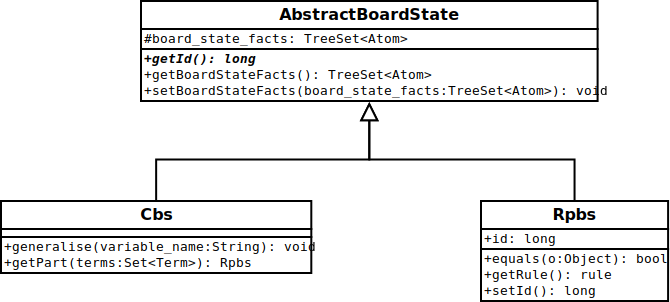
\includegraphics[width=\textwidth]{files/class_diagram/rpbs_cbs} 
\caption{Diagramme de classe des \class{\gls{Cbs}} et \class{\gls{Rpbs}}.} 
\label{img_diag_class_board_state}
\end{figure}

Les classes \class{\gls{Cbs}} et \class{\gls{Rpbs}} représentent respectivement un plateau et une sous configuration d'un plateau dans le format logique décrit dans la section \vref{subsection_representation_co}. 

\section{Analyse}

Le module d'analyse a un rôle de convertisseur. Le plateau fournit par l'environnement est un objet \texttt{\gls{BoardMatrix}} qui est transformé par le \emph{RuleBook} en un ensemble de \texttt{\gls{BoardMatrix}}, chacun correspondant à un coup possible. Ces objets sont ensuite convertit par l' \emph{analyseur conceptuel de base} en une représentation logique du premier ordre encapsulée dans des objets \texttt{\gls{CompleteBoardState}}.

L'\emph{analyseur conceptuel poussé} associe à chaque \texttt{\gls{CompleteBoardState}} des ensembles de \texttt{\gls{RelevantPartialBoardState}} correspondant aux formes reconnues dans le plateau.

Enfin, le couple \texttt{\gls{CompleteBoardState}} / liste de \texttt{\gls{RelevantPartialBoardState}} est déposé en mémoire à court terme sous la forme d'un object \texttt{\gls{Option_FOL}} avant de réveiller le module de raisonnement.

\subsection{Le \og RuleBook \fg{}}

\subsection{L'analyseur conceptuel de base}
Lors de chaque coup du jeu, l'analyseur conceptuel de base (comme défini dans la partie~\ref{def:analyseur de base}, page~\pageref{def:analyseur de base}), convertit donc, plus précisément, une instance de Choices en une instance the Choices\_FOL en se servant de classes qui modélisent la logique du premier ordre. 

Une première analyse d'un plateau en forme de matrice BoardMatrix permet l'analyseur de générer des faits logiques correspondants à la configuration du plateau. Cette liste de faits est ensuite rassemblée pour former une base de faits qui est stockée comme attribut de la classe CompleteBoardState correspondante à ce plateau. L'analyseur crée alors le pacquet Choices\_FOL correspondant au pacquet Choices de l'environnement en convertissant chaque plateau (BoardMatrix) de Choices en un plateau (CompleteBoardState) de Choices\_FOL. Elle passe ensuite ce pacquet à l'analyseur conceptuel poussé. 
\subsection{L'analyseur conceptuel poussé}
L'analyseur conceptuel poussé prend ce pacquet et, comme défini dans la partie~\ref{def:analyseur pousse}(page~\pageref{def:analyseur pousse}), associe des formes pertinantes (des RelevantPartialBoardState) récupérées par la mémoire, à chaque plateau présent dans ce pacquet. 

Les formes (RelevantPartialBoardState) récupérées de la mémoire correspondent à des règles logiques représentées comme une conjonction d'atomes, le dernier atome étant la conclusion de cette règle. Ici, l'hypothèse décrit une configuration (forme) pertinante, et la conclusion l'associe un id. Par exemple, le fait d'avoir pris un coin est représenté par la règle :

\textit{$isCorner() \wedge is(Mine) \Longrightarrow \_rpbs034$}. 

Ensuite, l'analyseur, en tant que moteur d'inférence, sature la base de faits de chaque plateau rencontré dans le pacquet Choices\_FOL par application de l'ensemble de ces règles. La reconnaissance des formes dans chacun de ces plateaux revient alors à rechercher l'homomorphisme de l'atome représentant l'id d'une forme pertinante dans la base de faits saturée de ce plateau. Une fois la reconnaissance (l'existance d'un homomorphisme) est établie, la règle ReleventPartialBoard state est ajoutée à la liste de formes pertinantes associée à ce plateau.

Pour résumer, le rôle de l'analyseur conceptuel poussé est donc de déterminer et d'ajouter cette liste de formes pertinantes à chaque plateau présent dans le pacquet Choices\_FOL. 

L'analyseur passe enfin ce pacquet enrichi à la mémoire et stimule le module de raisonnement afin de commencer son processus. 

\section{Raisonnement}

Etiam consequat, ante eget pellentesque placerat, lacus nisl facilisis lectus, nec luctus risus justo quis orci. Sed porttitor, neque quis ullamcorper venenatis, est augue convallis nisi, eu accumsan tortor magna nec urna. Aliquam erat volutpat. Nullam eget nulla nisl. Phasellus porta turpis id mauris eleifend rutrum. Suspendisse varius rhoncus magna, ut commodo ante lacinia at. Nullam viverra malesuada sapien eu luctus. 

Cras id lectus augue. Quisque varius sodales sapien eget gravida. Nulla a elit vel enim eleifend commodo ut et elit. Aliquam ornare, ante sit amet auctor commodo, tellus ipsum pellentesque eros, et gravida magna tortor quis nulla. Vestibulum diam quam, aliquet in lobortis fermentum, dignissim id purus. Nulla felis velit, rhoncus at vehicula id, varius vel odio. Quisque dolor nulla, mattis suscipit lacinia a, congue in lacus. Mauris tempor ultricies sapien eu adipiscing. Ut vestibulum libero vel nisi rutrum eu pellentesque orci commodo. 

Donec quis aliquam dolor. Mauris vitae diam sit amet urna pharetra blandit et non risus. Suspendisse velit lacus, suscipit eget feugiat a, vulputate sed sem. Ut placerat lectus sed leo vulputate at malesuada nisl cursus. Donec feugiat tempus quam, in commodo mi hendrerit sed. Ut ut mauris nisi, non ultricies lectus. Quisque lobortis ante eu dolor aliquet ut sagittis enim ultrices. Integer luctus facilisis ultricies. Nam non vestibulum turpis. Vestibulum dictum lacus quam, aliquet vulputate arcu. Donec quam nulla, condimentum vitae gravida sit amet, interdum at elit. Donec tempor eros at arcu rutrum ut tristique justo tincidunt. Nullam suscipit mauris et ligula pellentesque viverra vitae at nisi. 

\section{Mémoire}

\begin{frame}{Mémoire}{Interface Mémoire}
\begin{center}
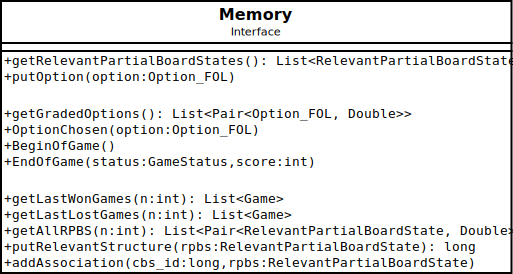
\includegraphics[width=0.7\textwidth]{img/implementation_memory/interface}
\end{center}
\end{frame}

\begin{frame}{Mémoire}{Persistance}
\begin{center}
\includegraphics[width=0.3\textwidth]{img/neo4j/neo4j_logo}
\end{center}
\begin{block}{Neo4j}
\begin{itemize}
\item Logiciel libre (GPLv3 / AGPLv3)
\item SGBD NoSQL orienté graphe
\item Respect des caractéristiques ACID
\item Multiple versions (embedded in Java)
\end{itemize}
\end{block}
\end{frame}

\begin{frame}{Mémoire}{Persistance}
\begin{block}{Élements}
\begin{itemize}
\item Noeud racine
\item Noeuds
\item Relations (orientées)
\item Types de relations
\item Attributs (Noeuds \& Relations)
\end{itemize}
\end{block}
\begin{block}{Comment typer les noeuds ?}
\begin{enumerate}
\item Créer un noeud \texttt{Maitre}
\item Créer une relation typée \texttt{Racine $\rightarrow$ Maitre}
\item Créer des relations typées \texttt{Maitre $\rightarrow$ Noeuds}
\end{enumerate}
\end{block}
\end{frame}

\chapter{Méthode de travail}

\section{Répartition des tâches}

Dans le but de pouvoir travailler séparément et de manière autonome sur chaque module lors de l'implémentation, nous avons rigoureusement travaillé les spécifications techniques et l'architecture globale de l'application. Les tâches de développement ont ensuite été  menées de manière parallèle par chacun des membres de l'équipe :

\begin{itemize}
\item Namrata était résponsable du module d'analyse,
\item Clément du raisonnement,
\item Thibaut de la mémoire,
\item et William de l'environnement et du serveur de jeu.
\end{itemize}   

Nous nous sommes réunis tout au long du développement pour assurer l'avancement global du projet et répondre aux interrogations de chacun.

\section{Outils utilisés}

\subsection{Gestionnaire de versions}
Tout au long du projet, nous avons utilisé \emph{git} : un gestionnaire de version décentralisé. Un tel outil permet la mise en commun des travaux, la gestion des versions et la gestion des \emph{merges}\footnote{Fusion de deux fichiers différents.}. 

\begin{center}
	\includegraphics[width=0.3\textwidth]{files/outils/git}	
\end{center}

Nous avons choisi \emph{git} pour plusieurs raisons :

\begin{itemize}
\item plutôt simple d'utilisation (par rapport à ses homologues comme \emph{SVN}),
\item hébergement gratuit via GitHub (sous condition de diffusion du code sous une licence libre),
\item \emph{git} est une solution libre sous licence \gls{GPLv2}.
\end{itemize}

\subsection{EtherPad, un éditeur de texte collaboratif}
\emph{EtherPad} se présente sous la forme d'un éditeur de texte léger permettant de faire un minimum de mise en page.

\begin{figure}[H]
	\includegraphics[width=\textwidth]{files/outils/etherpad_screenshot}	
	\caption{Aperçu de l'interface d'\emph{EtherPad} hébergé sur \emph{framapad} (site mis à disposition par Framasoft utilisant le code d'EtherPad).}
	\label{etherpad_screenshot}
\end{figure}

\begin{center}
\includegraphics[width=0.4\textwidth]{files/outils/etherpad}
\end{center}

L'interface d'\emph{EtherPad} se présente sous la forme d'une interface web (figure \ref{etherpad_screenshot}) où chaque utilisateur connecté possède une couleur. La singularité de cet outil réside dans le fait que toutes les modifications effectuées sur le pad sont visibles par tous en temps réel.

Un chat est également disponible ce qui facilite la collaboration entre les utilisateurs connectés.

Il est important de noter qu'\emph{EtherPad} est sous licence \gls{Apache v2}.

\subsection{Visualisation de graphes}

Pour débugger la base de données Neo4j, nous avons utilisé \emph{Gephi}, un utilitaire basé sur la \emph{NetBeans Platform}.

\begin{center}
\includegraphics[width=0.4\textwidth]{files/outils/gephi}
\end{center}

Il permet de visualiser et de manipuler des graphes. C'est un outil libre qui embarque quelques plugins dont un connecteur Neo4j permettant l'import de bases de données du SGBD.

\subsection{Outils de développement}
Voici une liste non exhaustive des outils que nous avons utilisés lors de nos développements :
\begin{description}
\item[Eclipse / NetBeans] Il s'agit des deux principaux EDI\footnote{Environnement de Développement Intégré} libres.
\item[Javadoc] Nous avons pris soin de documenter la totalité de notre code dans le but de rentre notre code réutilisable. Javadoc est aujourd'hui devenu un standard industriel utilisé par la majorité des développement Java.
\item[Log4j] Librairie Java libre qui permet la journalisation sous formes variées (stdout\footnote{Flux de sortie standard.}, fichiers de log, envoie de mail, etc.).
\item[YourKit Java Profiler] Afin de permettre d'optimiser certaines méthodes, nous avons utilisé cet outil en version d'évaluation (sous licence propriétaire). Il s'intègre parfaitement dans la plupart des environnement de développement.
\end{description}
\clearemptydoublepage
\begin{frame}{Optimisation}{Structures de données}

\end{frame}

\begin{frame}{Optimisation}{MultiThreading}

\end{frame}

\begin{frame}{Optimisation}{Autre}

\end{frame}
\clearemptydoublepage

\pagebreak
\addcontentsline{toc}{chapter}{Glossaire}
\printglossary

\end{document}
